\documentclass[conference]{IEEEtran}
\IEEEoverridecommandlockouts
% The preceding line is only needed to identify funding in the first footnote. If that is unneeded, please comment it out.
\usepackage{cite}
\usepackage{amsmath,amssymb,amsfonts}
\usepackage{algorithmic}
\usepackage{graphicx}
\usepackage{textcomp}
\usepackage{xcolor}
\usepackage{tabularx}
\usepackage{multirow}
\usepackage{graphics} % for pdf, bitmapped graphics files
\usepackage{subfig}
\usepackage{subcaption}
\usepackage{hyperref}
\usepackage{academicons}
\usepackage{xcolor}
\usepackage{listings}
\usepackage{tabularx} % Asegúrate de incluir este paquete

\usepackage{tikz}
\usetikzlibrary{shapes.geometric, arrows}

\usetikzlibrary{shapes.geometric, arrows}

\tikzstyle{startstop} = [rectangle, rounded corners, minimum width=3cm, minimum height=1cm,text centered, draw=black, fill=red!30]
\tikzstyle{process} = [rectangle, minimum width=3cm, minimum height=1cm, text centered, draw=black, fill=blue!30]
\tikzstyle{arrow} = [thick,->,>=stealth]


\def\BibTeX{{\rm B\kern-.05em{\sc i\kern-.025em b}\kern-.08em
		T\kern-.1667em\lower.7ex\hbox{E}\kern-.125emX}}

% Color Enlace
\definecolor{colorEnlace}{RGB}{0, 0, 0}
\hypersetup{
	colorlinks=true,
	linkcolor=colorEnlace,
	citecolor=colorEnlace,
	urlcolor=colorEnlace,
	pdfauthor={Davis Bremdow Salazar Roa},
	pdftitle={Sistemas Embebidos}
}
\definecolor{mybg}{rgb}{0.97,0.97,0.97}
\definecolor{mygray}{gray}{0.4}
\definecolor{mygreen}{rgb}{0,0.6,0}
\definecolor{myblue}{rgb}{0,0,0.8}
\definecolor{mypurple}{rgb}{0.58,0,0.82}
\definecolor{myred}{rgb}{0.7,0,0}

\lstdefinelanguage{MatlabEnhanced}{
	language=Matlab,
	morekeywords={[2]linspace,plot,title,xlabel,ylabel,legend,grid},
	morekeywords={[3]sin,cos,exp,log,sqrt},
	keywordstyle=\color{myblue}\bfseries,
	keywordstyle=[2]\color{mypurple},
	keywordstyle=[3]\color{myred},
	commentstyle=\color{mygreen}\itshape,
	stringstyle=\color{mygray},
	morecomment=[l]%
}

\lstset{
	language=MatlabEnhanced,
	backgroundcolor=\color{mybg},
	frame=single,
	basicstyle=\ttfamily\small,
	showstringspaces=false,
	numbers=none,              %
	xleftmargin=0pt,           %
	framexleftmargin=0pt,      
	framexrightmargin=0pt,
	framextopmargin=2pt,
	framexbottommargin=2pt,
	breaklines=true,
	tabsize=1,
}

% Control 
\usepackage{amsmath}
\begin{document}
	
	\title{Informe final - Amplificador Diferencial Retroalimentado}
	\author{
		\makebox[\textwidth][c]{\large\textbf{Universidad Nacional de San Antonio Abad del Cusco}}\\
		\makebox[\textwidth][c]{\normalsize\textit{Escuela profesional de Ingeniería Electrónica}}\\
		\makebox[\textwidth][c]{\normalsize\textit{Laboratorio de Circuitos Electrónicos III}}\\
		\and
		\IEEEauthorblockN{Ing. Milton Velasquez Curo}
		\IEEEauthorblockA{Ingeniero Electrónico \\
			Cusco, Perú \\
			milton.velasquez@unsaac.edu.pe}
		\and
		\IEEEauthorblockN{Ruth Juana Espino Puma - 185746}
		\IEEEauthorblockA{Estudiante de Ingeniería Electrónica \\
			Cusco, Perú \\
			184657@unsaac.edu.pe}
		\and
		\IEEEauthorblockN{Davis Bremdow Salazar Roa - 200353}
		\IEEEauthorblockA{Estudiante de Ingeniería Electrónica \\
			Cusco, Perú \\
			200353@unsaac.edu.pe}
	}
	
	\maketitle
	\begin{abstract}
		La modulación es un proceso fundamental en las telecomunicaciones que consiste en variar una o más propiedades de una señal portadora (como amplitud, frecuencia o fase) en función de una señal de información o mensaje. Este proceso permite transmitir información a largas distancias de manera eficiente, minimizando interferencias y aprovechando mejor el espectro de frecuencias. Existen varios tipos de modulación, entre ellos la modulación en amplitud (AM), frecuencia (FM) y fase (PM), cada una con características y usos específicos según las necesidades del sistema de comunicación.
		
		El índice de modulación es una medida que cuantifica la variación de la señal portadora en relación con la señal moduladora. Su importancia radica en que determina la eficiencia espectral, la calidad de la señal transmitida y el nivel de distorsión. Un índice bajo puede resultar en una señal débil o difícil de demodular, mientras que un índice muy alto puede causar sobre modulación y distorsión. En aplicaciones prácticas, la modulación es utilizada en radiodifusión (radio y televisión), comunicaciones satelitales, telefonía móvil, redes Wi-Fi, y sistemas de control industrial, donde el índice de modulación debe ser cuidadosamente ajustado para garantizar un rendimiento óptimo.
	\end{abstract}
	
	\begin{IEEEkeywords}
		Modulación, portadora, señal, índice de modulación, amplitud, frecuencia, fase, transmisión, espectro, distorsión.
	\end{IEEEkeywords}
	%% Contenido del documento
	
	\section{2. Análisis de Potencia}
	Para la generación de una señal modulada mediante la variación de amplitud es necesario el uso de 2 señales una que contenga la señal de información y otra de amplitud variable de gran frecuencia ello con la finalidad de poder trasladar la señal de información a una frecuencia que facilite su transmisión dentro del espectro radioeléctrico.
	
	Siendo así que dentro de este proceso además se puede realizar el análisis de potencia de ambas señales siendo esta una relación entre la energía/segundo utilizada por la señal de información y señal portadora encargada de realizar el desplazamiento en frecuencia.
	
	De forma general para poder realizar este análisis también se puede hacer uso de las ecuaciones \ref{eq:potencia-integral} y \ref{eq:potencia-suma} en las cuales se determinan la potencia de forma integral de la señal modulada resultante y la potencia en cada componente respectivamente.
	
	\begin{equation}
		P_{Cm} = \frac{1}{R_{L}} \int V_{Cm}^2(t)dt
		\label{eq:potencia-integral}
	\end{equation}
	\begin{equation}
		P_{Cm} = P_{c} + P_{BLS} + P_{BLI}
		\label{eq:potencia-suma}
	\end{equation}
	
	\subsection{\textbf{Calculo de la potencia}}
	Para el cálculo de potencia en función al código Matlab de ejemplo, solo fue necesario modificar la sección gráfica para adecuarla para el calculo de la potencia para cada caso, siendo esta modificación vista en el listing \ref{lst:potencia-matlab}
	
	\begin{lstlisting}[caption={Cálculo de Potencia}, label={lst:potencia-matlab}]
		clc, clear;
		%% Parametros de la simulacion
		fs = 10000;         % Frecuencia de muestreo (Hz)
		t = 0:1/fs:1-1/fs;  % Vector de tiempo (1 segundo)
		
		% Parametros de la senal portadora
		fc = 1000;          % Frecuencia de la portadora (Hz)
		Ac = 1;             % Amplitud de la portadora
		
		% Parametros de la senal moduladora
		fm = 100;           % Frecuencia de la moduladora (Hz)
		Am = 0.5;           % Amplitud de la moduladora
		ka = 2;           % Indice de modulacion (debe ser <= 1 para evitar sobremodulacion)
		
		%% Generacion de senales
		% Senal portadora
		portadora = Ac * cos(2*pi*fc*t);
		
		% Senal moduladora (coseno)
		moduladora = Am * cos(2*pi*fm*t);
		
		% Senal modulada AM
		modulada = Ac * (1 + ka*moduladora) .* cos(2*pi*fc*t);
		
		%% Analisis de potencia
		% Determinando Vcm(t)
		% Pc: Potencia portadora Pc = Ac^2/2;
		% Pbl: Potencia bandas laterales
		% Pcm: Potencia total
		% Pbls: Potencia en la banda superior
		% Pbli: Potencia en la banda inferior
		
		% Resistencia de potencia
		RL = 1;
		
		% Arreglo con los diferentes indices de modulacion
		indices = [0.3, 0.5, 0.7, 1, 1.2, 1.5, 1.8, 2];
		
		APc = [];
		APcm = [];
		APt = [];
		APbl = [];
		AEficiencia = [];
		
		for i = 1 : 1: length(indices)
		
		% Potencia en la portadora
		Pc = Ac^2/(2*RL);
		% Potencia en la banda lateral inferior
		Pbli = (indices(i)*Ac/2)^2/(2*RL);
		
		% Potencia en la banda lateral superior
		Pbls = (indices(i)*Ac/2)^2/(2*RL);
		
		% Potencia Total
		Pcm = Pc + Pbli + Pbls;
		Pt = (Ac^2/2)*(1 + indices(i)^2/2);
		
		% Potencia en las bandas laterales
		Pbl = Pbli + Pbls; 
		
		% Eficiencia de la modulacion
		eficiencia = Pbl/Pcm;
		
		APc = [APc, Pc];
		APcm = [APcm, Pcm];
		APt = [APt, Pt];
		APbl = [APbl, Pbl];
		AEficiencia = [AEficiencia, eficiencia];
		end
		
		figure;
		subplot(221);
		stem(indices, APc);
		title('Potencia de la portadora');
		
		subplot(222);
		stem(indices, APcm);
		title('Potencia total');
		
		subplot(223);
		stem(indices, APbl);
		title('Potencia en las bandas laterales');
		
		subplot(224)
		stem(indices, AEficiencia);
		title('Eficiencia de la modulacion');
		
		figure;
		stem(indices, APt);
	\end{lstlisting}
	
	\subsection{Comparación entre los valores teóricos y simulados}
	
	Para el cálculo de la potencia total o en el caso de la ecuación \ref{eq:potencia-suma} se debe conocer la expresión de la señal modulada resultante, siendo para este caso que tal expresión se detalla como el producto de la señal moduladora y portadora, obteniendo como resultado la expresión \ref{eq:modulada-analitica}
	
	\begin{equation}
		V_{AM}(t) = V_cCos\omega_ct + \frac{mV_c}{2}Cos(\omega_c + \omega_m)t + \frac{mV_c}{2}Cos(\omega_c - \omega_m)t 
		\label{eq:modulada-analitica}
	\end{equation}
	
	Siendo así que la potencia estaría siendo definida para el caso de una señal sinuidal estaría siendo definida por \ref{eq:potencia-senial} y en la cual se puede apreciar una relación de la amplitud con las coeficientes de Fourier para el calculo de la potencia.
	
	\begin{equation}
		P = \frac{A^2}{2}
		\label{eq:potencia-senial}
	\end{equation}
	
	Además en la relación \ref{eq:modulada-analitica} y \ref{eq:potencia-senial} se puede apreciar una dependencia de la potencia frente al índice de modulación, la amplitud de la portadora y la resistencia de potencia utilizada para la disipación por un factor de $\frac{1}{R_L}$ definida en \ref{eq:potencia-integral}, siendo para el caso de esta experiencia que este tendrá un valor de un $1\Omega$.
	
	Finalmente al realizar la comparación de este calculo de forma teórica y simulada, no se pudo apreciar cierta diferencia debido a que el este calculo se realiza mediante el empleo de simples operaciones matemáticas las cuales no difieren mucho al no ser de orden complejo.
	
	\begin{table}[]
		\centering
		\begin{tabular}{|c|c|c|}
			\hline
			\textbf{Índice de Modulación} & \textbf{Manual} & \multicolumn{1}{l|}{\textbf{Simulado}} \\ \hline
			0.5                           & 0.5625          & 0.5625                                 \\ \hline
			1                             & 0.75            & 0.75                                   \\ \hline
			1.5                           & 1.0625          & 1.0625                                 \\ \hline
		\end{tabular}
		\label{tab:comparacion-potencia}
	\end{table}
	
	En la tabla \ref{tab:comparacion-potencia} se puede apreciar los resultados obtenidos para cada caso, observándose una relación proporcional directa entre el índice de modulación y la potencia total resultante.
	
	\subsection{\textbf{Relación entre $P_{total}$, $P_c$, $P_{Bl}$ frente $K_a$}}
	
	En la modificación al código mostrada en \ref{lst:potencia-matlab} también se definieron el calculo de 
	\begin{itemize}
		\item Potencia Total ($P_{cm}$)
		\item Potencia Portadora ($P_c$)
		\item Potencia Bandas Laterales ($P_{BL}$)
	\end{itemize}
	
	frente al indice de modulación, lo cual permitió facilito realizar el análisis de la señal modula frente al cambio repentino del índice de modulación $K_a$.
	
	\begin{figure}[h]
		\centering
		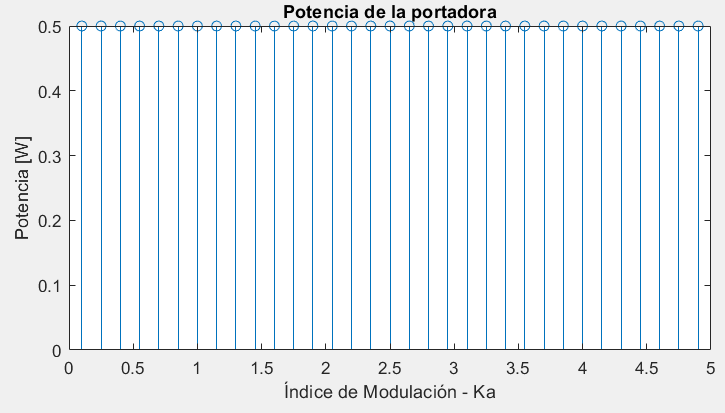
\includegraphics[width=0.4\textwidth]{media/potencia-portadora}
		\caption{Potencia de la portadora respecto al índice de modulación}
		\label{fig:potencia-portadora}
	\end{figure}
	
	\begin{figure}[h]
		\centering
		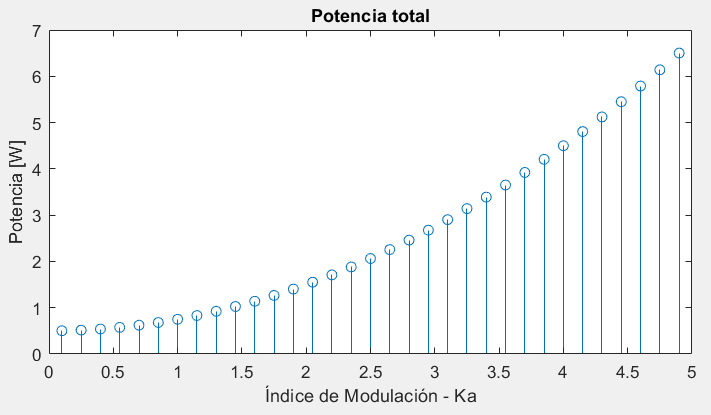
\includegraphics[width=0.4\textwidth]{media/potencia-total}
		\caption{Evolución de la potencia total respecto al índice de modulación}
		\label{fig:potencia-total}
	\end{figure}
	
	\begin{figure}[h]
		\centering
		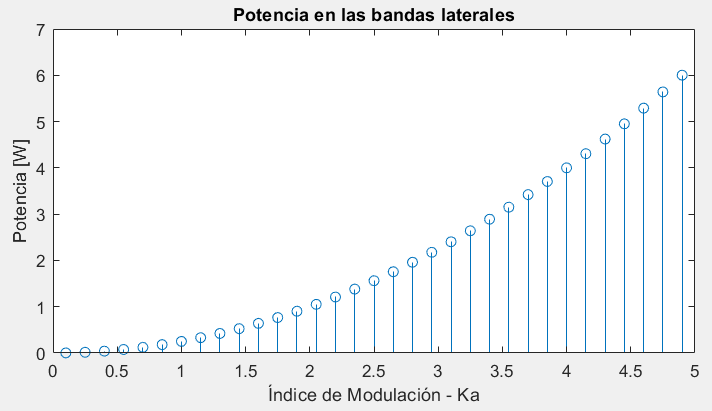
\includegraphics[width=0.4\textwidth]{media/potencia-laterales}
		\caption{Potencia en las bandas laterales respecto al índice de modulación}
		\label{fig:potencia-laterales}
	\end{figure}
	
	\subsection{\textbf{Relaciones no lineales}}
	En las figuras \ref{fig:potencia-portadora}, \ref{fig:potencia-total} y \ref{fig:potencia-laterales} se pudo apreciar la evolución de la energía disipada por segundo de la señal modulada frente el cambio del indice de modulación en el rango entre 0.1 hasta 2 en el cual se puede apreciar 2 comportamiento claramente diferenciados, siendo uno de ello el calculo de la potencia de la portadora que se mantiene constante debido a que no guarda una relación directa con el índice $K_a$ y por otro en las figuras consecuentes \ref{fig:potencia-total} y \ref{fig:potencia-laterales} la relación entre potencia e índice de modulación contempla una relación exponencial creciente conforme $K_a$ aumenta su valor.
	
	Relación justificada debido a que el índice $K_a$ al definirse como la amplitud de la señal resultante del producto no lineal de la modulación es elevado la cuadrado definiendo la no lineal de la respuesta graficada.
	
	\section{\textbf{Modulación con Señal Compleja}}
	
	La señal compleja a utilizar para este punto se define en \ref{eq:moduladora-compleja} y en la cual se define 2 señales sinusoidales de diferente frecuencia y amplitud, en función al código de ejemplo propuesto se modifico tal expresión para hacer uso de una sola amplitud al factorizar 0.3 a toda la expresión, obteniendo de tal forma la expresión definida en \ref{eq:moduladora-compleja-1} y cual se implemento en matlab.
	
		
	\begin{equation}
		m(t) = 0.3\cos(2\pi 100 t) + 0.2\cos(2\pi 200 t)
		\label{eq:moduladora-compleja}
	\end{equation}
	
	\begin{equation}
		m(t) = 0.3(\cos(2\pi 100 t) + 0.67\cos(2\pi 200 t))
		\label{eq:moduladora-compleja-1}
	\end{equation}
	
	El código Matlab modificado para este fin se aprecia en el listing \ref{lst:} y en la cual solo se tuvo que modificar la parte superior del código en la sección para la generación de señales y los parámetros de la señal moduladora.
	
	\begin{lstlisting}[caption={Moduladora compleja}, label={lst:moduladora-compleja}, numbers=none]
		%% Parametros de la simulacion
		fs = 10000;         % Frecuencia de muestreo (Hz)
		t = 0:1/fs:1-1/fs;  % Vector de tiempo (1 segundo)
		
		% Parametros de la senal portadora
		fc = 1000;          % Frecuencia de la portadora (Hz)
		Ac = 1;             % Amplitud de la portadora
		
		% Parametros de la senal moduladora
		fm = 100;           % Frecuencia de la moduladora (Hz)
		Am = 0.3;           % Amplitud de la moduladora
		ka = 2;           % Indice de modulacion (debe ser <= 1 para evitar sobremodulacion)
		
		%% Generacion de senales
		% Senal portadora
		portadora = Ac * cos(2*pi*fc*t);
		
		% Senal moduladora (coseno)
		moduladora = Am * ( cos(2*pi*fm*t) + 0.67*cos(2*pi*2*fm*t) );
		
		% Senal modulada AM
		modulada = Ac * (1 + ka*moduladora) .* cos(2*pi*fc*t);
	\end{lstlisting}
	
	\subsection{\textbf{Análisis del espectro}}
	En el espectro de la modulación de tono complejo se pudo apreciar en la parte de la moduladora 2 señales destacadas con amplitud máxima en las frecuencia de 100, 200 y sus equivalentes negativos respectivamente y la cual se justifica por medio de la definición del tono complejo, por otro lado en la señal portadora en comparación al primer ejemplo, no se apreciar cambios significativos en su espectro.
	
	Finalmente en la figura \ref{fig:espectro-complejo} se pudo apreciar que el espectro de la señal modulada se vio alterado debido a las componentes en frecuencia de la señal moduladora apreciándose 5 impulsos: 1 correspondiente a la portadora, 2 debido la componente de 100 Hz y 2 a causa de la componente de 200 Hz.
	
	\begin{figure}[h]
		\centering
		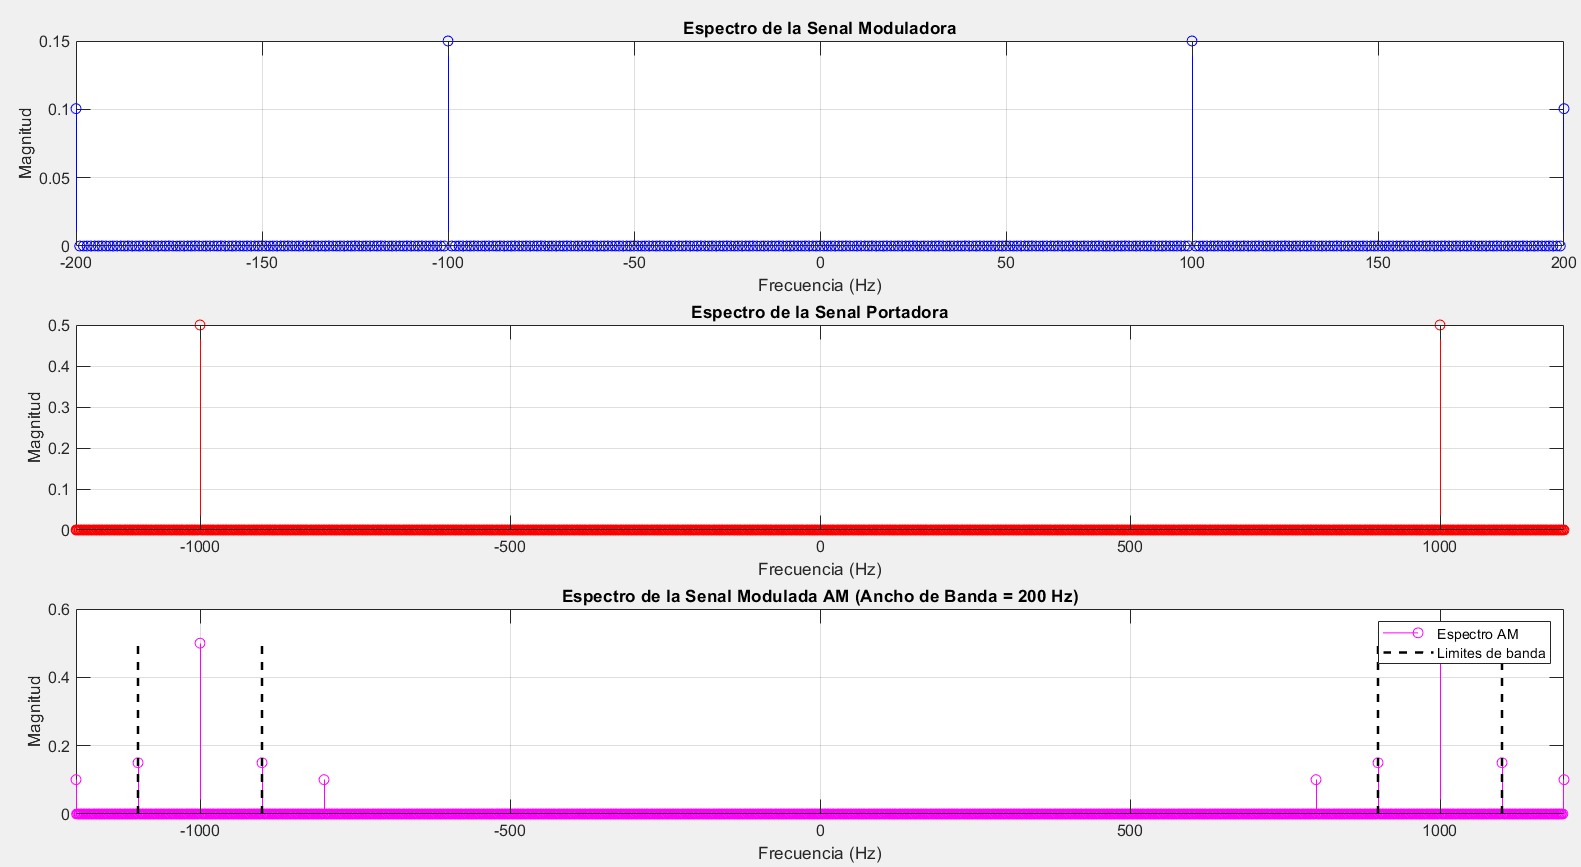
\includegraphics[width=0.4\textwidth]{media/espectro-complejo}
		\caption{Espectro de la modulación de tono complejo}
		\label{fig:espectro-complejo}
	\end{figure}
	
	Por otro lado en la respuesta en el dominio del tiempo se pudo apreciar una misma correlación entre la respuesta o salida del producto entre la moduladora y la portadora.
	
	\subsection{\textbf{Ancho de banda de la señal}}
	
	Debido a las componentes en frecuencia de la moduladora, el ancho de banda de la señal modulada resultante también se vio afectado y/o modificado y lo cual se justifica mediante la variación en el espectro de la señal, siendo así que el nuevo ancho de banda será la diferencia entre la banda lateral superior e inferior de mayor frecuencia.
	
	\begin{align}
		BW &= 1200 - 800 \\
		BW &= 400 Hz
	\end{align}
	
	\subsection{Eficiencia moduladora de tono y tono complejo}
	
	\section{Cuestionario - preguntas conceptuales}
	
	\subsection{\textbf{Explique el fenómeno de sobremodulación y sus consecuencias prácticas}}
	
	La sobremodulación es un fenómeno que ocurre cuando el índice de modulación el cual relación al amplitud de señal de información y el de la portadora es mayor 1 indicando que la amplitud de la señal de información es mayor al de la señal portadora, provocando que exista una superposición de la señal moduladora resultante impidiendo o dificultando la recuperación de la señal de información.
	
	\subsection{\textbf{¿Cómo afectaría a la señal AM un cambio de fase en la portadora?}}
	
	Debido a que en una señal AM se propaga la información en la envolvente o en la amplitud de la señal modulada, un cambio de fase no afecta significativamente a la información transmitida debido a que la amplitud no es afectada por el cambio de fase, simplemente se tendría una desplazamiento en el tiempo de la señal (generando un atraso o retardo según el valor del desfase).
	
	\section{Cuestionario - Problemas}
	
	\subsection{\textbf{Modulación AM de una señal}}
	Se requiere una modulación con las siguientes características $A_c = 10V; f_c = 1MHz; m(t) = 2\cos(2\pi5*10^3t); k_a = 0.4;$ y con las cuales se desea realizar una modulación AM.
	\subsection{\textbf{Expresión completa de s(t)}}
	
	Para la obtención de la señal modulada es necesario realizar el producto entre la señal moduladora y portadora, siendo el resultado de esta la que nos brindará la expresión completa de s(t), definiendo la portadora, se tiene:
	
	\begin{equation}
		m(t) = 2\cos(2\pi5*10^3t)
		\label{eq:moduladora}	
	\end{equation}
	
	\begin{equation}
		A_cCos(2\pi10^6t)
		\label{eq:portadora}
	\end{equation}
	
	Siendo la formula general para la obtención de la señal modulada la que se expresa en \ref{eq:moduladora-general} la cual hace uso directamente del indice de modulación y del producto entre la moduladora y la portadora.
	
	\begin{equation}
		s(t) = Ac(1 + K_am(t))cos(2\pi f_ct)
		\label{eq:moduladora-general}
	\end{equation}
	
	Luego de aplicar esta relación el resultado obtenido muestra la señal moduladora desplazada en frecuencia una cantidad equivalente al de la portadora obtenido la relación \ref{eq:} perteneciente a s(t).
	
	\begin{equation}
		s(t) = 10cos(2\pi10^6t) + 4cos(2\pi10^6 + 2\pi5*10^3)t + 4cos(2\pi10^6 - 2\pi5*10^3)t
	\end{equation}
	
	\subsection{Calculo de la potencia total de la señal s(t)}
	
	Para el calculo de la potencia solo basta con elevar al cuadrada la amplitud de cada componente sinusoidal y dividirlo entre 2, el resultado de la operación \ref{eq:potencia-total-propuesto-1}
	
	\begin{align}
		P &= \frac{10^2}{2} + \frac{4^2}{2} + \frac{4^2}{2}\\
		P &= 66 [w] \\
		\label{eq:potencia-total-propuesto-1}
	\end{align}
	
	\subsection{Sistema AM en matlab}
	Para realizar la grabación de voz mediante Matlab y luego  proceder con el procesamiento de la misma, se puede hacer de la herramienta \textbf{audiorecorder} el cual permite manipular señales físicas mediante un objeto con el cual se controlan los parámetros de la grabación como la frecuencia de muestreo y la duración de la grabación.
	
	Esta función definida en el bloque de código de forma simple permite la grabación, reproducción y grabado del audio en un formato de archivo .wav, el cual puede ser manipulado en otra área de trabajo.
	
	\begin{lstlisting}[caption={Manipulación de audio con audiorecorder}, label={lst:grabacion-audio}]
		recObj = audiorecorder;
		recordblocking(recObj, 5);
		play(recObj);
		
		y = getaudiodata(recObj); 
		plot(y);
		
		Fs = 8000;
		audiowrite('grabacion.wav', y, Fs);
		
		
		% Recuperar el archivo en matlab
		
		[y, Fs] = audioread('grabacion.wav');
		sound(y, Fs);
		
	\end{lstlisting}
	
	Para este caso el audio generado tiene una duración de 5 segundos con un total de 40000 muestras para la frecuencia de muestreo de 8000, además esta misma se puede procesar mediante la función \textbf{audioread} con la finalidad de esta experiencia su modulación AM.
	
	La modulación de esta señal se muestra en la siguiente ventana de código en la cual se cambio la frecuencia de muestreo a una adecuada para la señal y se hizo uso de la misma portadora para su traslado en frecuencia.
	
	\begin{lstlisting}[caption={Modulaciòn de la señal de audio}, numbers=none]
		%% Parametros de la simulacion
		Fs = 8000;         % Frecuencia de muestreo (Hz)
		t = 0 : 1/Fs : 1;  % Vector de tiempo (1 segundo)
		
		% Parametros de la senal portadora
		fc = 1000;          % Frecuencia de la portadora (Hz)
		Ac = 1;             % Amplitud de la portadora
		
		% Parametros de la senal moduladora
		fm = 100;           % Frecuencia de la moduladora (Hz)
		Am = 0.5;           % Amplitud de la moduladora
		ka = 2;           
		
		%% Generacion de senales
		% senal portadora
		portadora = Ac * cos(2*pi*fc*t);
		
		% senal moduladora (coseno)
		[y, Fs] = audioread('grabacion.wav');
		sound(y, Fs);
		moduladora = y(8000:16000);
		
		% senal modulada AM
		modulada = Ac * (1 + ka*moduladora) .* cos(2*pi*fc*t);
	\end{lstlisting}
	
	Donde grabacion.wav es el archivo de audio generado.
	
	\subsection{Espectro de potencia de la señal modulada}
	
	Como resultado de la modulación se puede apreciar que los componentes principales de esta señal se encuentran entre los 120 a 200 Hz y el resultado de su modulación y respuesta en el tiempo y frecuencia se puede apreciar en la figuras \ref{fig:modulacion-audio-tiempo}  y \ref{fig:modulacion-audio-frecuencia} respectivamente las cuales muestran gráficamente este proceso.
	
	\begin{figure}[h]
		\centering
		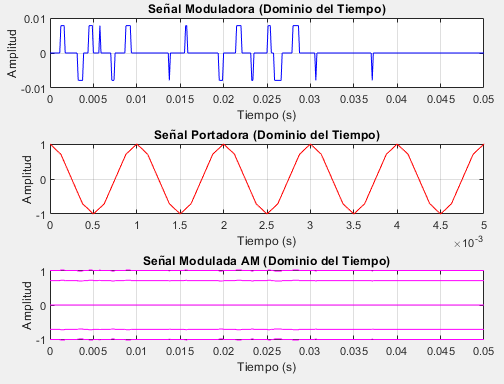
\includegraphics[width=0.4\textwidth]{media/modulacion-audio-tiempo}
		\caption{Respuesta de la modulación AM en el tiempo de la señal de audio}
		\label{fig:modulacion-audio-tiempo}
	\end{figure}
	
	En la señal de frecuencia debido a los diferentes componentes sinusoidales que componen tal señal es más elaborado crear un análisis matemático para representar toda sus componentes en frecuencia.
	
	\begin{figure}[h]
		\centering
		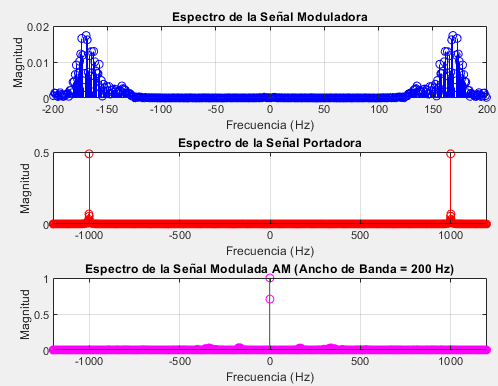
\includegraphics[width=0.4\textwidth]{media/modulacion-audio-frecuencia}
		\caption{Respuesta en frecuencia de la modulación AM de la señal de audio}
		\label{fig:modulacion-audio-frecuencia}
	\end{figure}
	
	
	
	\subsection{Demodulación  AM}
	Para realizar la demodulación de la señal se considerara un método basado en la DSBSC la cual consiste en volver a multiplicar la señal modulada por la misma portadora y luego aplicar un filtro pasa bajo para solamente recuperar las componentes en frecuencia de banda base con la cual se genero la señal.
	
	Además cabe resaltar que este proceso a nivel de simulación brinda una respuesta cercana y/o muy fiable de la información modulada, sin embargo este proceso en una implementación física es difícil de conseguir una alta fidelidad debido a las dificultes de conseguir 2 osciladores con las mismas características, optando por demodulación asincrona basada en los detectores de envolvente.
	
	Finalmente en las figuras \ref{fig:senial-modulada} y \ref{fig:senial-demodulada} se tienen el proceso de modulación a la señal de audio y demodulación luego del filtro respectivamente.
	
	\begin{figure}[h]
		\centering
		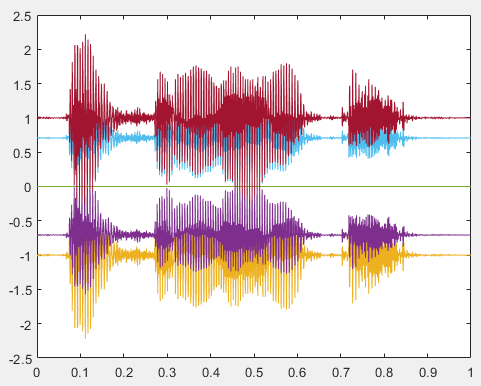
\includegraphics[width=0.4\textwidth]{media/senial-modulada}
		\caption{Señal de Audio modulada}
		\label{fig:senial-modulada}
	\end{figure}
	
	\begin{figure}[h]
		\centering
		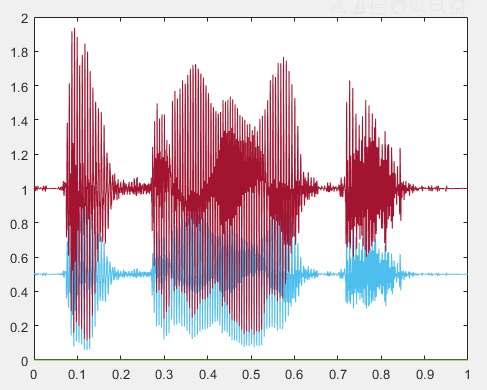
\includegraphics[width=0.4\textwidth]{media/senial-demodulada}
		\caption{Señal de Audio demodulada}
		\label{fig:senial-demodulada}
	\end{figure}
		
	\section{Conclusiones}
	
	\begin{itemize}
		\item La modulación AM es inherentemente ineficiente pero sencilla de implementar.
		\item El índice de modulación debe controlarse cuidadosamente para evitar distorsión.
		\item MATLAB permite visualizar claramente los efectos en tiempo y frecuencia.
		\item El análisis espectral es fundamental para entender sistemas de comunicaciones.
	\end{itemize}
	
	\bibliographystyle{IEEEtran}
	\bibliography{biblio}
\end{document}
